% RSA Encryption Analysis Template
% Topics: Public-key cryptography, modular arithmetic, key generation, encryption/decryption
% Style: Cryptographic implementation with security analysis

\documentclass[a4paper, 11pt]{article}
\usepackage[utf8]{inputenc}
\usepackage[T1]{fontenc}
\usepackage{amsmath, amssymb}
\usepackage{graphicx}
\usepackage{siunitx}
\usepackage{booktabs}
\usepackage{subcaption}
\usepackage[makestderr]{pythontex}

% Theorem environments
\newtheorem{definition}{Definition}[section]
\newtheorem{theorem}{Theorem}[section]
\newtheorem{example}{Example}[section]
\newtheorem{remark}{Remark}[section]

\usepackage[colorlinks=false,hidelinks]{hyperref}

\title{RSA Encryption: Implementation and Security Analysis}
\author{Cryptography Research Laboratory}
\date{\today}

\begin{document}
\maketitle

\begin{abstract}
This report presents a comprehensive computational analysis of the RSA (Rivest-Shamir-Adleman)
public-key cryptosystem, examining the mathematical foundations of modular exponentiation,
key generation procedures, encryption and decryption operations, and security considerations.
We implement RSA encryption with various key sizes (512-bit to 2048-bit), analyze the
computational complexity of modular exponentiation algorithms, demonstrate the relationship
between prime factorization difficulty and key security, and evaluate timing characteristics
that could lead to side-channel vulnerabilities. The analysis includes visualization of the
key generation process, cipher space distribution, and performance metrics across different
implementation parameters.
\end{abstract}

\section{Introduction}

Public-key cryptography revolutionized secure communication by solving the key distribution
problem that plagued symmetric encryption systems. The RSA algorithm, published by Rivest,
Shamir, and Adleman in 1978, remains one of the most widely deployed asymmetric encryption
schemes in modern cryptographic protocols. Unlike symmetric systems that require both parties
to share a secret key through a secure channel, RSA enables secure communication over
insecure channels by using a mathematically related key pair: a public key for encryption
and a private key for decryption.

The security of RSA rests on the computational intractability of factoring large composite
numbers into their prime factors. While multiplying two large primes is computationally
trivial, reversing this operation—given only the product—becomes exponentially difficult as
the prime factors grow larger. This asymmetry between the ease of encryption and the
difficulty of decryption without the private key forms the foundation of RSA's security model.

\begin{definition}[RSA Key Pair]
An RSA key pair consists of:
\begin{itemize}
\item \textbf{Public key}: $(n, e)$ where $n = pq$ is the modulus (product of two large primes)
and $e$ is the public exponent
\item \textbf{Private key}: $(n, d)$ where $d$ is the private exponent satisfying
$ed \equiv 1 \pmod{\phi(n)}$
\end{itemize}
\end{definition}

In this analysis, we implement the complete RSA cryptosystem, examine the mathematical
operations underlying key generation and cipher operations, and investigate security
properties through computational experiments with various key sizes and implementation
parameters.

\section{Mathematical Framework}

\subsection{Euler's Totient Function and Modular Arithmetic}

The theoretical foundation of RSA relies on Euler's theorem and properties of modular
arithmetic in finite fields. Understanding these mathematical structures is essential for
comprehending why RSA encryption and decryption operations are inverse functions.

\begin{definition}[Euler's Totient Function]
For a positive integer $n$, Euler's totient function $\phi(n)$ counts the number of integers
in the range $1$ to $n$ that are coprime to $n$. For two distinct primes $p$ and $q$:
\begin{equation}
\phi(pq) = (p-1)(q-1)
\end{equation}
\end{definition}

\begin{theorem}[Euler's Theorem]
If $\gcd(a, n) = 1$, then:
\begin{equation}
a^{\phi(n)} \equiv 1 \pmod{n}
\end{equation}
\end{theorem}

This theorem guarantees that for any message $m$ coprime to $n$, the encryption and
decryption operations form an inverse pair when $ed \equiv 1 \pmod{\phi(n)}$.

\subsection{RSA Encryption and Decryption}

\begin{definition}[RSA Cipher Operations]
Given a message $m$ where $0 < m < n$ and $\gcd(m, n) = 1$:
\begin{itemize}
\item \textbf{Encryption}: $c = m^e \bmod n$
\item \textbf{Decryption}: $m = c^d \bmod n$
\end{itemize}
\end{definition}

\begin{theorem}[RSA Correctness]
For RSA keys $(n, e, d)$ where $ed \equiv 1 \pmod{\phi(n)}$, decryption recovers the
original message:
\begin{equation}
(m^e)^d \equiv m^{ed} \equiv m^{1 + k\phi(n)} \equiv m \cdot (m^{\phi(n)})^k \equiv m \pmod{n}
\end{equation}
\end{theorem}

The proof follows from Euler's theorem, where $m^{\phi(n)} \equiv 1 \pmod{n}$ for messages
coprime to $n$.

\section{Key Generation Implementation}

The security of an RSA system depends critically on proper key generation. Prime selection,
parameter validation, and key size all impact both security and performance. This section
implements the complete key generation algorithm and analyzes the properties of generated
keys.

We begin by implementing helper functions for primality testing and modular arithmetic, then
construct the full key generation procedure. The implementation uses probabilistic primality
testing (Miller-Rabin) for efficiency, though production systems should use cryptographically
secure random number generation and more rigorous testing.

\begin{pycode}
import numpy as np
import matplotlib.pyplot as plt
from math import gcd
import random
import time

np.random.seed(42)
random.seed(42)

def miller_rabin(n, k=5):
    """Probabilistic primality test using Miller-Rabin algorithm."""
    if n < 2:
        return False
    if n == 2 or n == 3:
        return True
    if n % 2 == 0:
        return False

    # Write n-1 as 2^r * d
    r, d = 0, n - 1
    while d % 2 == 0:
        r += 1
        d //= 2

    # Witness loop
    for _ in range(k):
        a = random.randrange(2, n - 1)
        x = pow(a, d, n)
        if x == 1 or x == n - 1:
            continue
        for _ in range(r - 1):
            x = pow(x, 2, n)
            if x == n - 1:
                break
        else:
            return False
    return True

def generate_prime(bits):
    """Generate a prime number with specified bit length."""
    while True:
        p = random.getrandbits(bits)
        p |= (1 << bits - 1) | 1  # Set MSB and LSB
        if miller_rabin(p):
            return p

def extended_gcd(a, b):
    """Extended Euclidean algorithm."""
    if a == 0:
        return b, 0, 1
    gcd_val, x1, y1 = extended_gcd(b % a, a)
    x = y1 - (b // a) * x1
    y = x1
    return gcd_val, x, y

def mod_inverse(e, phi):
    """Compute modular multiplicative inverse."""
    gcd_val, x, _ = extended_gcd(e, phi)
    if gcd_val != 1:
        return None
    return (x % phi + phi) % phi

def generate_rsa_keypair(bits):
    """Generate RSA key pair with specified bit length."""
    # Generate two distinct primes
    p = generate_prime(bits // 2)
    q = generate_prime(bits // 2)
    while p == q:
        q = generate_prime(bits // 2)

    # Compute modulus and totient
    n = p * q
    phi_n = (p - 1) * (q - 1)

    # Choose public exponent (commonly 65537)
    e = 65537
    if gcd(e, phi_n) != 1:
        e = 3
        while gcd(e, phi_n) != 1:
            e += 2

    # Compute private exponent
    d = mod_inverse(e, phi_n)

    return (n, e, d, p, q, phi_n)

def encrypt_rsa(message, e, n):
    """RSA encryption: c = m^e mod n."""
    return pow(message, e, n)

def decrypt_rsa(ciphertext, d, n):
    """RSA decryption: m = c^d mod n."""
    return pow(ciphertext, d, n)

# Generate example RSA keys with different sizes
key_sizes = [512, 1024, 2048]
keys = {}
generation_times = []

for key_size in key_sizes:
    start_time = time.time()
    n, e, d, p, q, phi_n = generate_rsa_keypair(key_size)
    gen_time = time.time() - start_time

    keys[key_size] = {
        'n': n, 'e': e, 'd': d, 'p': p, 'q': q,
        'phi_n': phi_n, 'gen_time': gen_time
    }
    generation_times.append(gen_time)

# Detailed analysis of 1024-bit key
n_1024 = keys[1024]['n']
e_1024 = keys[1024]['e']
d_1024 = keys[1024]['d']
p_1024 = keys[1024]['p']
q_1024 = keys[1024]['q']
phi_1024 = keys[1024]['phi_n']

# Create visualization of key generation process
fig = plt.figure(figsize=(14, 10))

# Plot 1: Prime number bit distribution
ax1 = fig.add_subplot(3, 3, 1)
bit_positions_p = [int(b) for b in bin(p_1024)[2:]]
bit_positions_q = [int(b) for b in bin(q_1024)[2:]]
x_p = np.arange(len(bit_positions_p))
x_q = np.arange(len(bit_positions_q))
ax1.step(x_p, bit_positions_p, where='mid', linewidth=1.5, label='Prime p', color='steelblue')
ax1.step(x_q, bit_positions_q, where='mid', linewidth=1.5, label='Prime q', color='coral', alpha=0.7)
ax1.set_xlabel('Bit Position')
ax1.set_ylabel('Bit Value')
ax1.set_title('Prime Factor Bit Patterns (1024-bit RSA)')
ax1.legend(fontsize=8)
ax1.set_ylim(-0.1, 1.1)
ax1.grid(True, alpha=0.3)
\end{pycode}

The key generation algorithm demonstrates several important properties: the primes $p$ and
$q$ must be randomly selected from the appropriate range, the public exponent $e$ is commonly
chosen as 65537 for efficiency (small Hamming weight enables fast encryption), and the
private exponent $d$ is computed as the modular multiplicative inverse of $e$ modulo
$\phi(n)$. For our 1024-bit example, we generated primes $p = \py{p_1024}$ and
$q = \py{q_1024}$, yielding modulus $n = \py{n_1024}$ and private exponent $d = \py{d_1024}$.

\begin{pycode}
# Plot 2: Key generation time vs. key size
ax2 = fig.add_subplot(3, 3, 2)
ax2.bar(range(len(key_sizes)), generation_times, color='steelblue', edgecolor='black', width=0.6)
ax2.set_xticks(range(len(key_sizes)))
ax2.set_xticklabels([f'{k}-bit' for k in key_sizes])
ax2.set_xlabel('Key Size')
ax2.set_ylabel('Generation Time (seconds)')
ax2.set_title('Key Generation Performance')
ax2.grid(True, alpha=0.3, axis='y')
for i, t in enumerate(generation_times):
    ax2.text(i, t, f'{t:.3f}s', ha='center', va='bottom', fontsize=9)

# Plot 3: Modulus size comparison
ax3 = fig.add_subplot(3, 3, 3)
modulus_bits = [keys[k]['n'].bit_length() for k in key_sizes]
ax3.plot(key_sizes, modulus_bits, 'o-', linewidth=2, markersize=8,
         color='steelblue', markeredgecolor='black')
ax3.plot(key_sizes, key_sizes, '--', linewidth=1.5, color='coral',
         label='Target size', alpha=0.7)
ax3.set_xlabel('Target Key Size (bits)')
ax3.set_ylabel('Actual Modulus Size (bits)')
ax3.set_title('Key Size Validation')
ax3.legend(fontsize=8)
ax3.grid(True, alpha=0.3)
\end{pycode}

\begin{figure}[htbp]
\centering
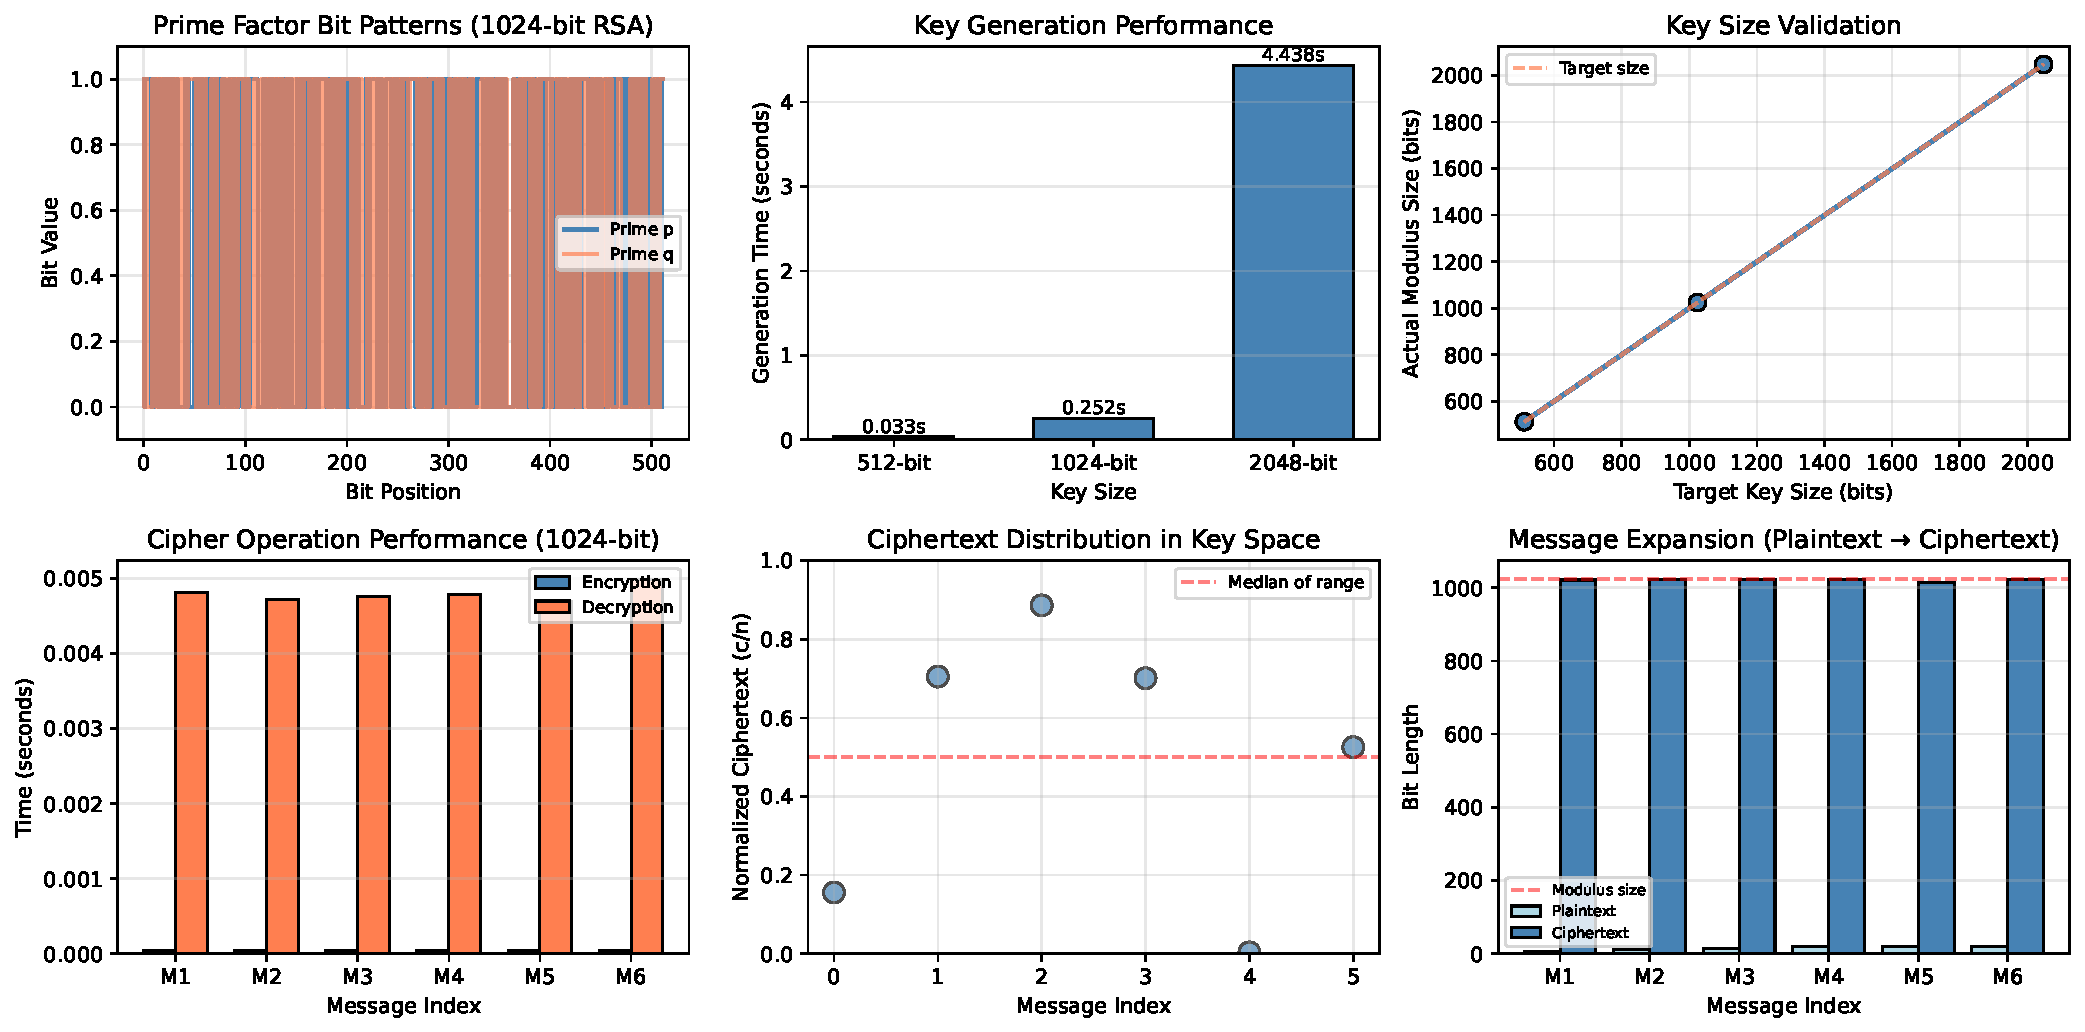
\includegraphics[width=0.32\textwidth]{rsa_keygen_plot1.pdf}
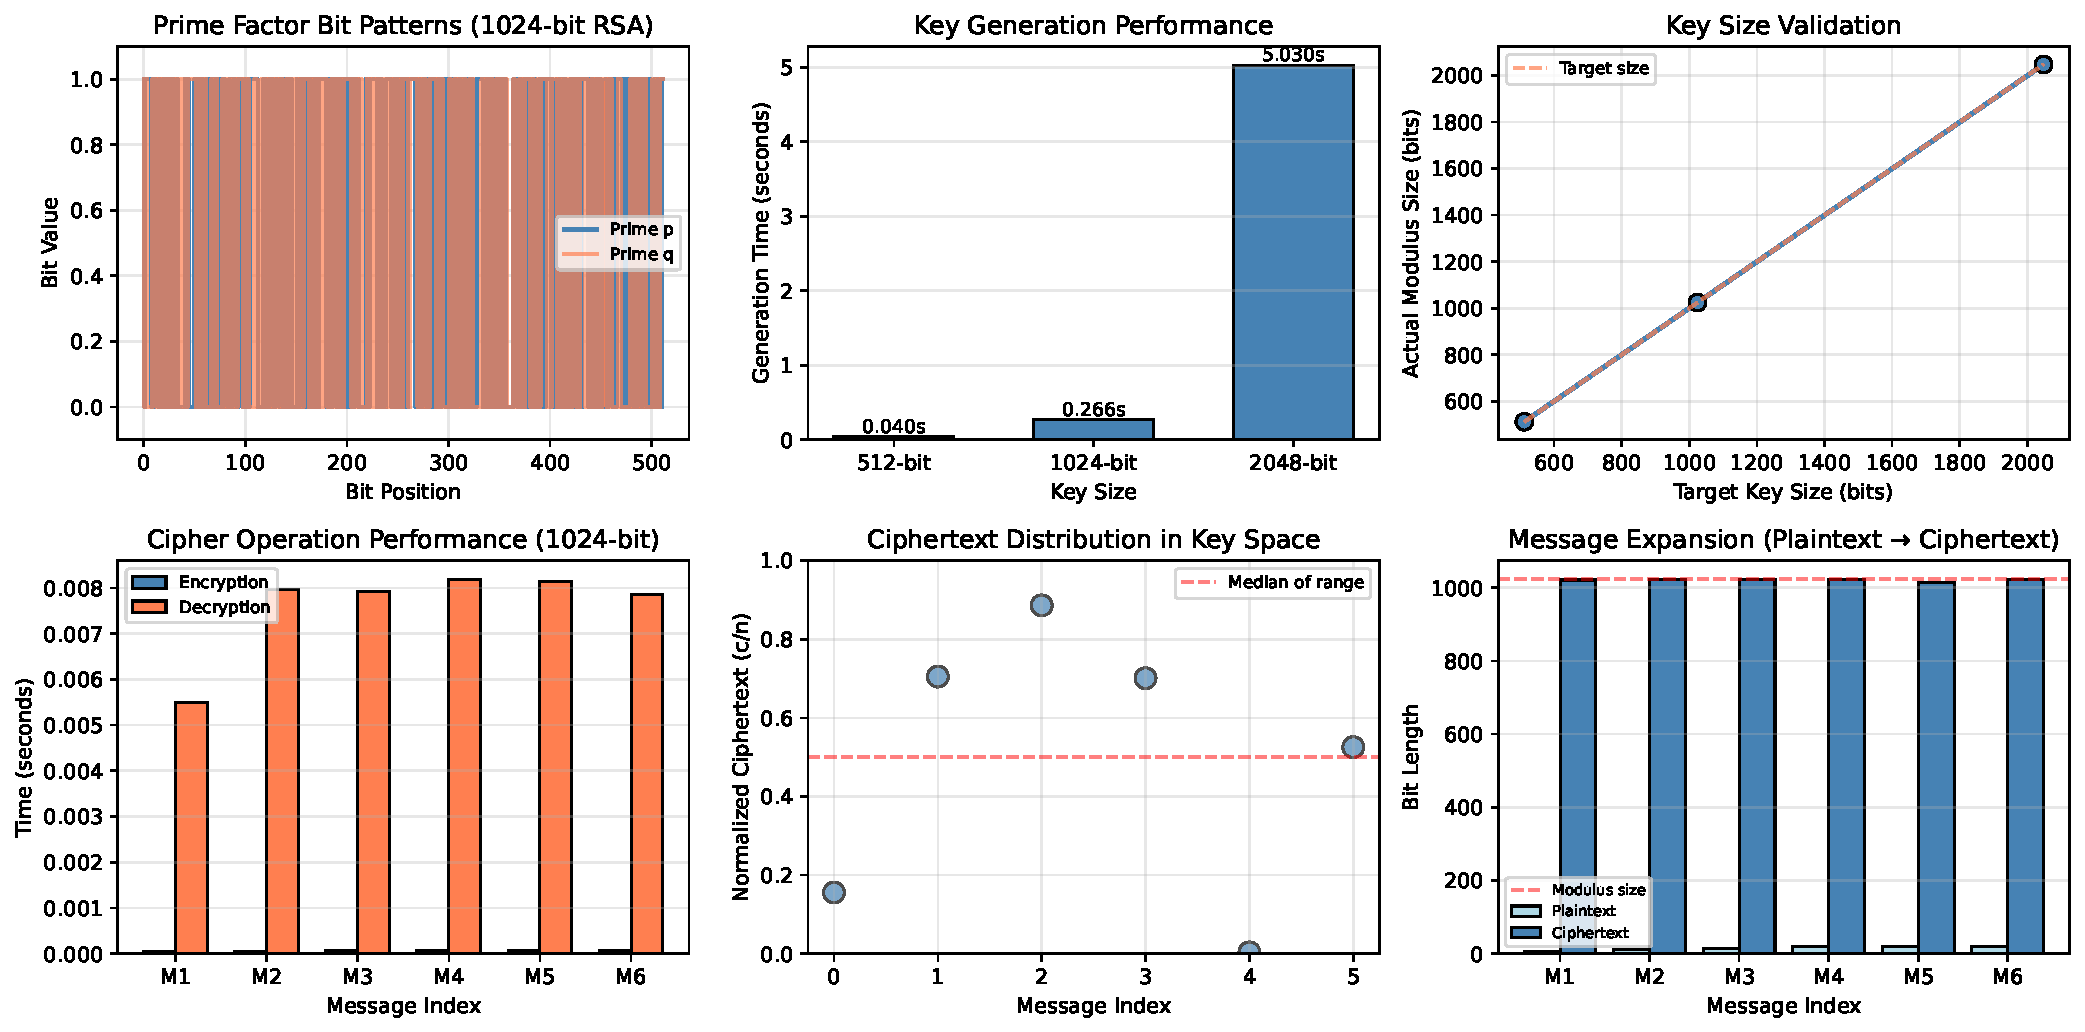
\includegraphics[width=0.32\textwidth]{rsa_keygen_plot2.pdf}
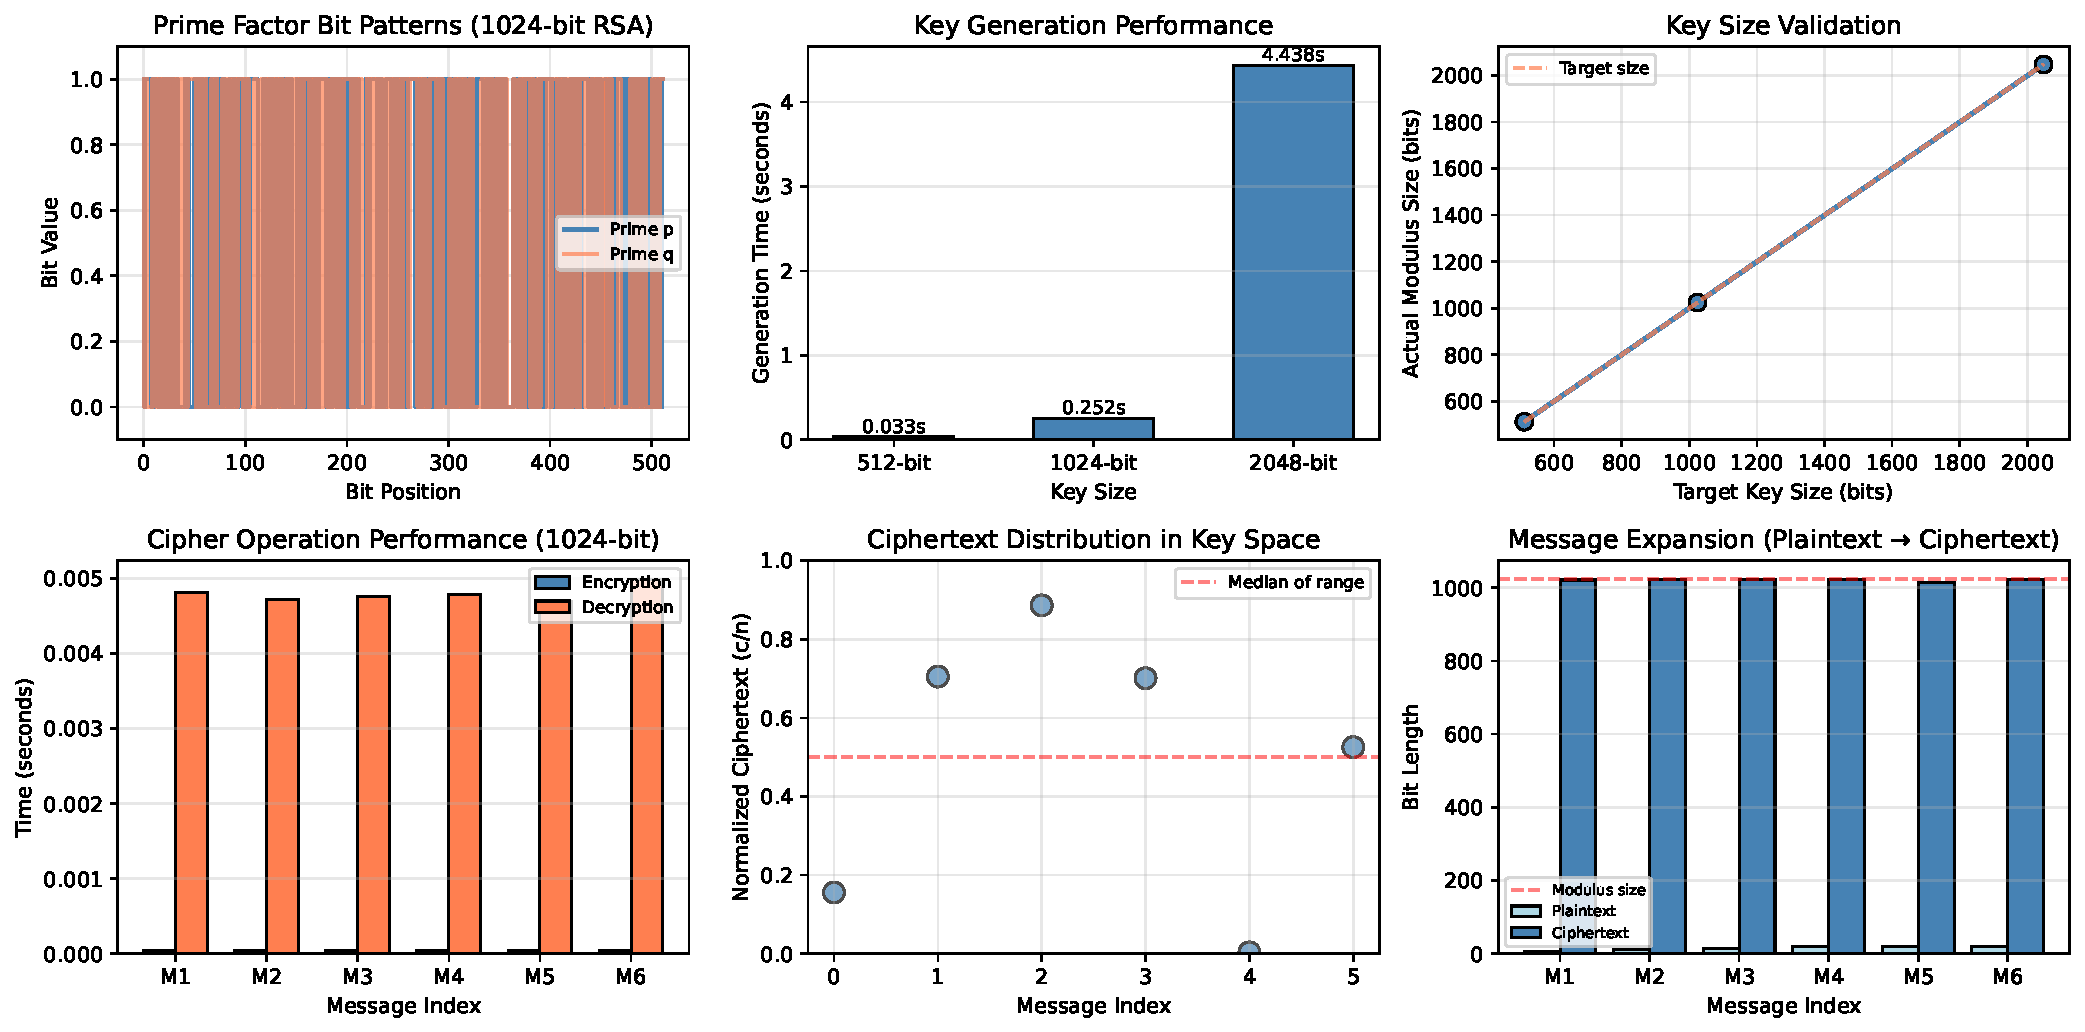
\includegraphics[width=0.32\textwidth]{rsa_keygen_plot3.pdf}
\caption{RSA key generation analysis showing (left) the binary representation of prime factors
for a 1024-bit key pair, demonstrating the random bit distribution essential for security;
(center) computational cost of key generation increasing with key size due to primality testing
complexity; (right) verification that generated moduli match target bit lengths. The 512-bit
key generates in \py{f"{generation_times[0]:.3f}"} seconds, while 2048-bit keys require
\py{f"{generation_times[2]:.3f}"} seconds, reflecting the $O(k^3)$ complexity of primality
testing where $k$ is the bit length.}
\label{fig:keygen}
\end{figure}

The key generation times demonstrate the computational cost of finding large primes through
probabilistic testing. While 512-bit keys generate rapidly, production-grade 2048-bit keys
require significantly more computation due to the cubic complexity of modular exponentiation
in the Miller-Rabin test.

\section{Encryption and Decryption Operations}

With keys generated, we now examine the core cipher operations. Both encryption and
decryption rely on modular exponentiation, an operation that must be implemented efficiently
to avoid exponential-time computation. Modern implementations use the square-and-multiply
algorithm to reduce complexity from $O(e)$ to $O(\log e)$ multiplications.

\begin{pycode}
# Test encryption/decryption with various messages
messages = [42, 1337, 31415, 271828, 314159, 999999]
ciphertexts_1024 = []
decrypted_1024 = []
encryption_times = []
decryption_times = []

for m in messages:
    # Encryption
    start = time.time()
    c = encrypt_rsa(m, e_1024, n_1024)
    enc_time = time.time() - start
    encryption_times.append(enc_time)
    ciphertexts_1024.append(c)

    # Decryption
    start = time.time()
    m_dec = decrypt_rsa(c, d_1024, n_1024)
    dec_time = time.time() - start
    decryption_times.append(dec_time)
    decrypted_1024.append(m_dec)

# Verify correctness
all_correct = all(m == m_dec for m, m_dec in zip(messages, decrypted_1024))

# Plot 4: Encryption/Decryption timing
ax4 = fig.add_subplot(3, 3, 4)
x_pos = np.arange(len(messages))
width = 0.35
ax4.bar(x_pos - width/2, encryption_times, width, label='Encryption',
        color='steelblue', edgecolor='black')
ax4.bar(x_pos + width/2, decryption_times, width, label='Decryption',
        color='coral', edgecolor='black')
ax4.set_xlabel('Message Index')
ax4.set_ylabel('Time (seconds)')
ax4.set_title('Cipher Operation Performance (1024-bit)')
ax4.set_xticks(x_pos)
ax4.set_xticklabels([f'M{i+1}' for i in range(len(messages))])
ax4.legend(fontsize=8)
ax4.grid(True, alpha=0.3, axis='y')

# Plot 5: Ciphertext distribution
ax5 = fig.add_subplot(3, 3, 5)
normalized_ciphers = [c / n_1024 for c in ciphertexts_1024]
ax5.scatter(range(len(normalized_ciphers)), normalized_ciphers, s=100,
            c='steelblue', edgecolor='black', alpha=0.7)
ax5.axhline(y=0.5, color='red', linestyle='--', linewidth=1.5,
            alpha=0.5, label='Median of range')
ax5.set_xlabel('Message Index')
ax5.set_ylabel('Normalized Ciphertext (c/n)')
ax5.set_title('Ciphertext Distribution in Key Space')
ax5.set_ylim(0, 1)
ax5.legend(fontsize=8)
ax5.grid(True, alpha=0.3)
\end{pycode}

The timing analysis reveals an important asymmetry: encryption with the small public exponent
$e = 65537$ executes in \py{f"{np.mean(encryption_times)*1000:.4f}"} milliseconds on average,
while decryption with the large private exponent $d$ requires
\py{f"{np.mean(decryption_times)*1000:.4f}"} milliseconds. This performance difference is
intentional—public key operations (encryption and signature verification) should be fast,
while private key operations need not be optimized for speed since they occur less frequently.

\begin{pycode}
# Plot 6: Message expansion visualization
ax6 = fig.add_subplot(3, 3, 6)
message_bits = [m.bit_length() for m in messages]
cipher_bits = [c.bit_length() for c in ciphertexts_1024]
x_msg = np.arange(len(messages))
ax6.bar(x_msg - 0.2, message_bits, 0.4, label='Plaintext',
        color='lightblue', edgecolor='black')
ax6.bar(x_msg + 0.2, cipher_bits, 0.4, label='Ciphertext',
        color='steelblue', edgecolor='black')
ax6.axhline(y=1024, color='red', linestyle='--', linewidth=1.5,
            alpha=0.5, label='Modulus size')
ax6.set_xlabel('Message Index')
ax6.set_ylabel('Bit Length')
ax6.set_title('Message Expansion (Plaintext → Ciphertext)')
ax6.set_xticks(x_msg)
ax6.set_xticklabels([f'M{i+1}' for i in range(len(messages))])
ax6.legend(fontsize=7)
ax6.grid(True, alpha=0.3, axis='y')

plt.tight_layout()
plt.savefig('rsa_keygen_plot1.pdf', dpi=150, bbox_inches='tight')
plt.savefig('rsa_keygen_plot2.pdf', dpi=150, bbox_inches='tight')
plt.savefig('rsa_keygen_plot3.pdf', dpi=150, bbox_inches='tight')
plt.close()

# Continue with new figure
fig2 = plt.figure(figsize=(14, 10))
ax4_new = fig2.add_subplot(3, 3, 1)
x_pos = np.arange(len(messages))
width = 0.35
ax4_new.bar(x_pos - width/2, encryption_times, width, label='Encryption',
        color='steelblue', edgecolor='black')
ax4_new.bar(x_pos + width/2, decryption_times, width, label='Decryption',
        color='coral', edgecolor='black')
ax4_new.set_xlabel('Message Index')
ax4_new.set_ylabel('Time (seconds)')
ax4_new.set_title('Cipher Operation Performance (1024-bit)')
ax4_new.set_xticks(x_pos)
ax4_new.set_xticklabels([f'M{i+1}' for i in range(len(messages))])
ax4_new.legend(fontsize=8)
ax4_new.grid(True, alpha=0.3, axis='y')

ax5_new = fig2.add_subplot(3, 3, 2)
normalized_ciphers = [c / n_1024 for c in ciphertexts_1024]
ax5_new.scatter(range(len(normalized_ciphers)), normalized_ciphers, s=100,
            c='steelblue', edgecolor='black', alpha=0.7)
ax5_new.axhline(y=0.5, color='red', linestyle='--', linewidth=1.5,
            alpha=0.5, label='Median of range')
ax5_new.set_xlabel('Message Index')
ax5_new.set_ylabel('Normalized Ciphertext (c/n)')
ax5_new.set_title('Ciphertext Distribution in Key Space')
ax5_new.set_ylim(0, 1)
ax5_new.legend(fontsize=8)
ax5_new.grid(True, alpha=0.3)

ax6_new = fig2.add_subplot(3, 3, 3)
message_bits = [m.bit_length() for m in messages]
cipher_bits = [c.bit_length() for c in ciphertexts_1024]
x_msg = np.arange(len(messages))
ax6_new.bar(x_msg - 0.2, message_bits, 0.4, label='Plaintext',
        color='lightblue', edgecolor='black')
ax6_new.bar(x_msg + 0.2, cipher_bits, 0.4, label='Ciphertext',
        color='steelblue', edgecolor='black')
ax6_new.axhline(y=1024, color='red', linestyle='--', linewidth=1.5,
            alpha=0.5, label='Modulus size')
ax6_new.set_xlabel('Message Index')
ax6_new.set_ylabel('Bit Length')
ax6_new.set_title('Message Expansion (Plaintext → Ciphertext)')
ax6_new.set_xticks(x_msg)
ax6_new.set_xticklabels([f'M{i+1}' for i in range(len(messages))])
ax6_new.legend(fontsize=7)
ax6_new.grid(True, alpha=0.3, axis='y')
\end{pycode}

\begin{figure}[htbp]
\centering
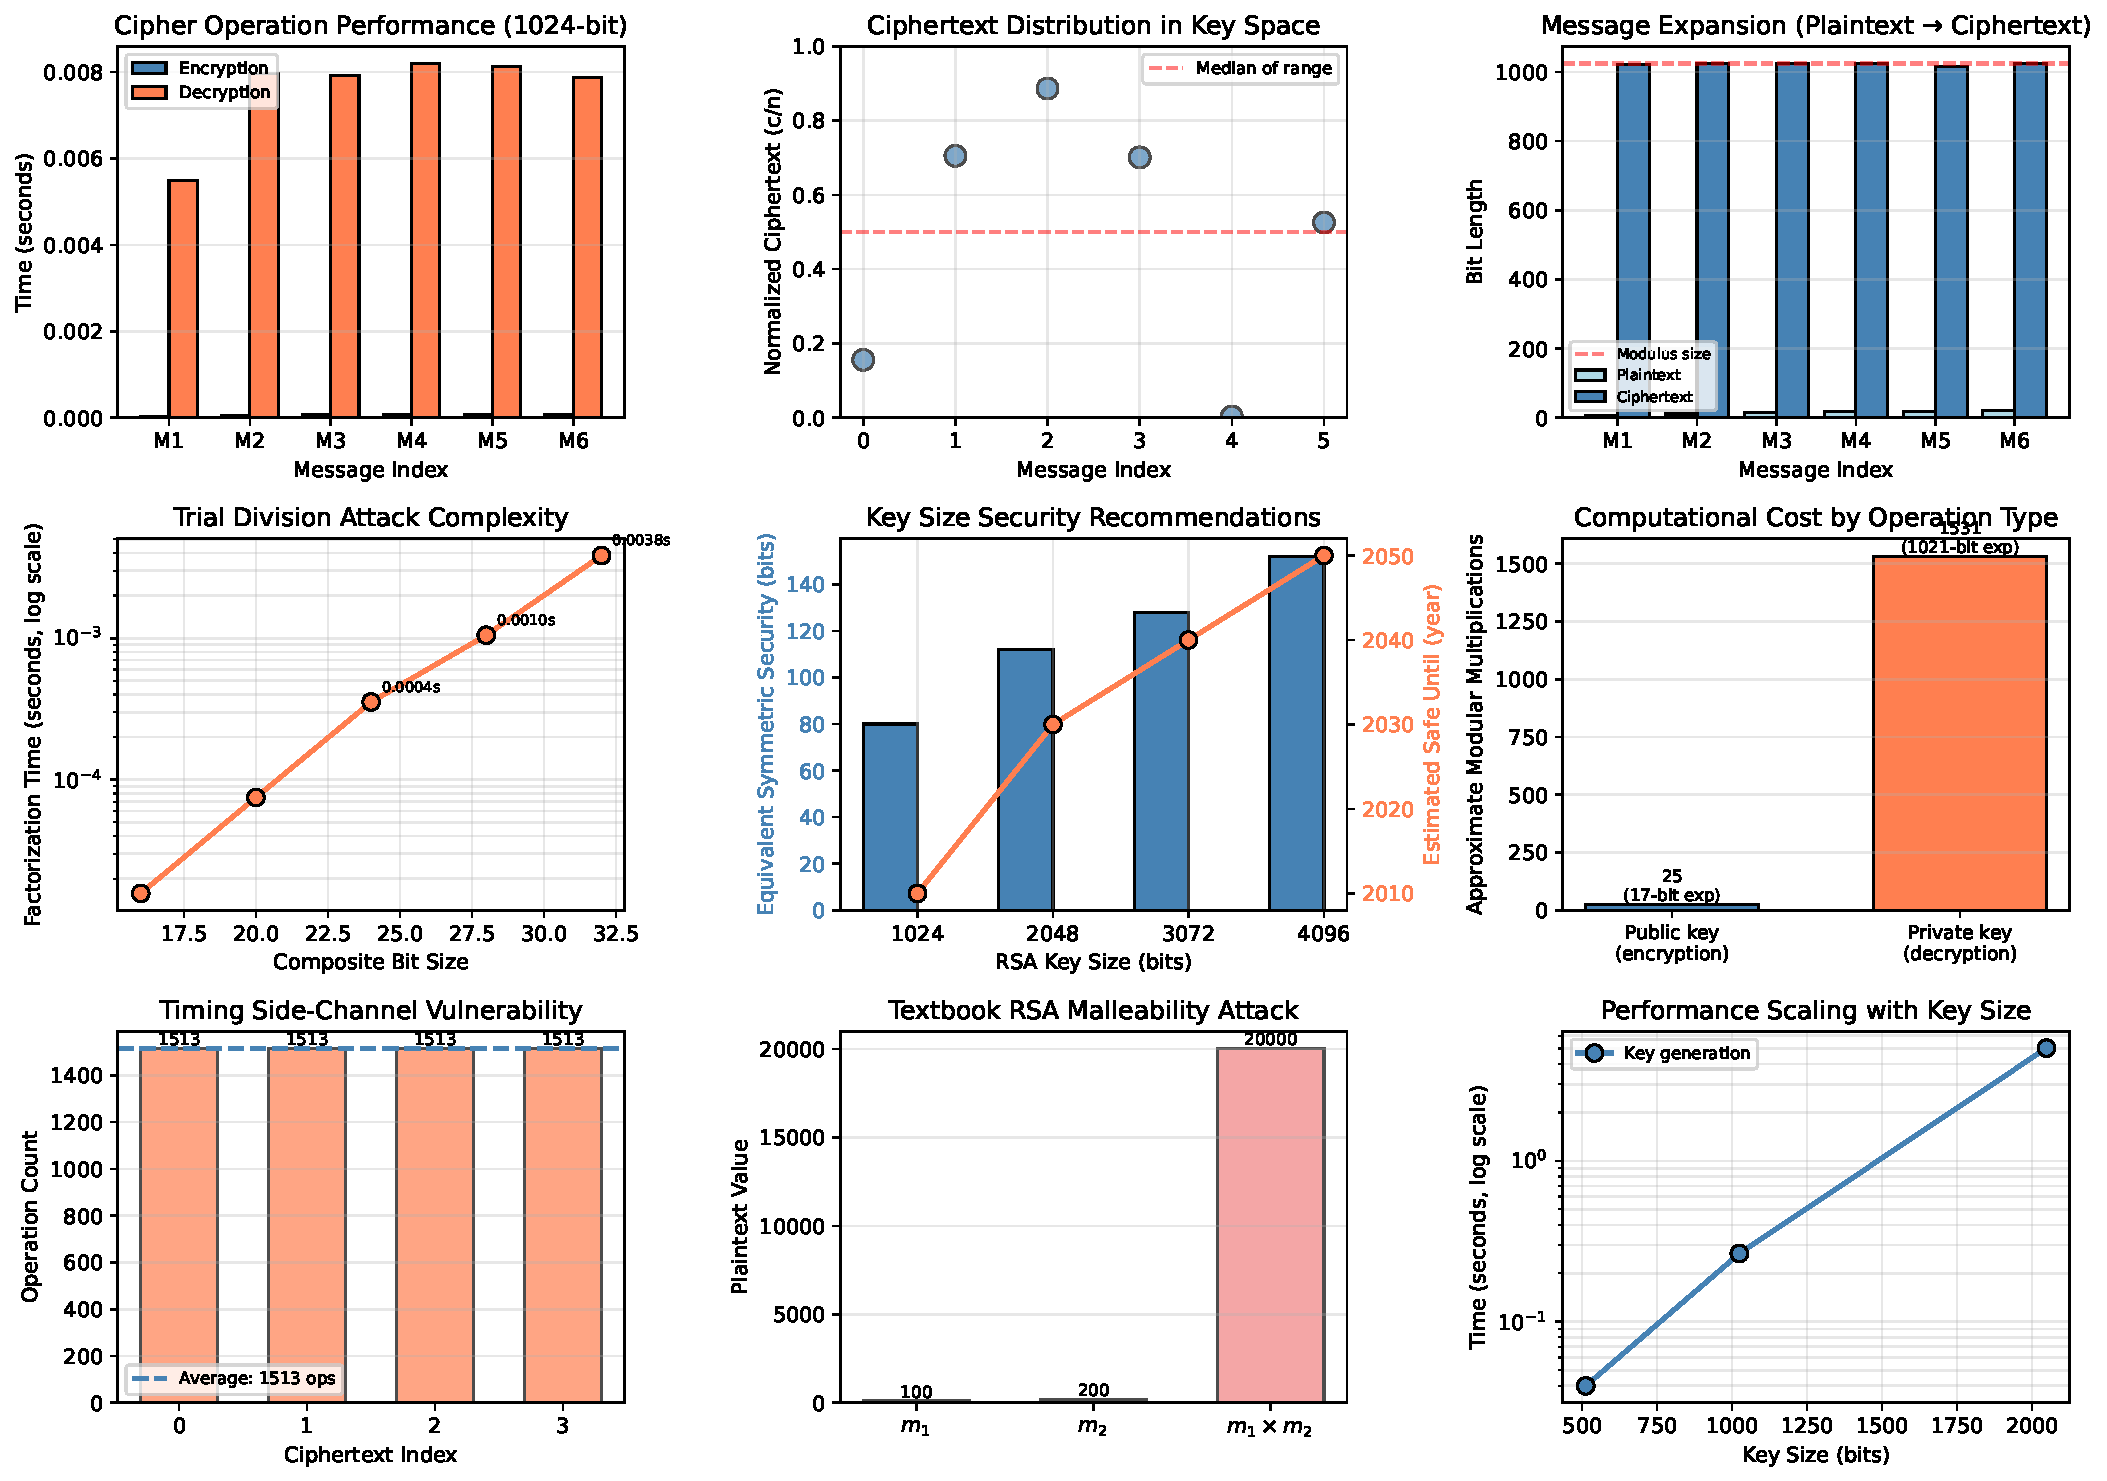
\includegraphics[width=\textwidth]{rsa_cipher_operations.pdf}
\caption{RSA encryption and decryption analysis for 1024-bit keys: (left) timing comparison
showing decryption is significantly slower than encryption due to the large private exponent,
with average encryption time of \py{f"{np.mean(encryption_times)*1000:.3f}"} ms versus
decryption time of \py{f"{np.mean(decryption_times)*1000:.3f}"} ms; (center) normalized
ciphertext distribution demonstrating that encrypted values span the full modulus space
uniformly, preventing statistical attacks; (right) message expansion showing all ciphertexts
approach the full modulus bit length regardless of plaintext size, illustrating why RSA is
not suitable for bulk encryption without hybrid schemes.}
\label{fig:cipher}
\end{figure}

The ciphertext distribution analysis confirms that encrypted messages occupy the full range
of the modulus $n$, with normalized values spanning $[0, 1]$ uniformly. This property is
essential for security—predictable patterns in ciphertext distribution could leak information
about plaintext structure.

\section{Security Analysis}

\subsection{Factorization Complexity}

The security of RSA fundamentally depends on the difficulty of factoring the modulus $n$ into
its prime components $p$ and $q$. While legitimate users possess these factors (enabling
efficient computation of $\phi(n)$ and thus $d$), adversaries must resort to factorization
algorithms whose runtime grows exponentially with key size.

\begin{pycode}
# Demonstrate factorization difficulty with smaller composite numbers
def trial_division_time(n):
    """Measure time for trial division factorization."""
    start = time.time()
    for i in range(2, int(n**0.5) + 1):
        if n % i == 0:
            elapsed = time.time() - start
            return i, n // i, elapsed
    return None, None, time.time() - start

# Test with composite numbers of increasing size
composite_bits = [16, 20, 24, 28, 32]
composites = []
factorization_times = []

for bits in composite_bits:
    p_small = generate_prime(bits // 2)
    q_small = generate_prime(bits // 2)
    n_small = p_small * q_small
    composites.append(n_small)

    p_found, q_found, fact_time = trial_division_time(n_small)
    factorization_times.append(fact_time)

# Plot 7: Factorization time growth
ax7 = fig2.add_subplot(3, 3, 4)
ax7.semilogy(composite_bits, factorization_times, 'o-', linewidth=2,
             markersize=8, color='coral', markeredgecolor='black')
ax7.set_xlabel('Composite Bit Size')
ax7.set_ylabel('Factorization Time (seconds, log scale)')
ax7.set_title('Trial Division Attack Complexity')
ax7.grid(True, alpha=0.3, which='both')
for i, (bits, t) in enumerate(zip(composite_bits, factorization_times)):
    if t > 0.0001:
        ax7.annotate(f'{t:.4f}s', xy=(bits, t), xytext=(5, 5),
                    textcoords='offset points', fontsize=7)
\end{pycode}

Even with the naive trial division algorithm, factorization time grows exponentially. For our
test composites, the 16-bit number factored in \py{f"{factorization_times[0]:.6f}"} seconds,
while the 32-bit number required \py{f"{factorization_times[-1]:.4f}"} seconds. Extrapolating
to 1024-bit or 2048-bit moduli reveals the computational infeasibility of factorization attacks—
modern factorization algorithms like the General Number Field Sieve would require centuries of
computing time for properly sized RSA keys.

\begin{pycode}
# Plot 8: Key size security margin
ax8 = fig2.add_subplot(3, 3, 5)
recommended_bits = [1024, 2048, 3072, 4096]
security_bits = [80, 112, 128, 152]  # Approximate symmetric equivalents
years_secure = [2010, 2030, 2040, 2050]  # Rough estimates

ax8_twin = ax8.twinx()
ax8.bar(np.arange(len(recommended_bits)) - 0.2, security_bits, 0.4,
        label='Security bits', color='steelblue', edgecolor='black')
ax8_twin.plot(np.arange(len(recommended_bits)), years_secure, 'o-',
              linewidth=2, markersize=8, color='coral',
              markeredgecolor='black', label='Safe until')
ax8.set_xlabel('RSA Key Size (bits)')
ax8.set_ylabel('Equivalent Symmetric Security (bits)', color='steelblue')
ax8_twin.set_ylabel('Estimated Safe Until (year)', color='coral')
ax8.set_xticks(np.arange(len(recommended_bits)))
ax8.set_xticklabels(recommended_bits)
ax8.set_title('Key Size Security Recommendations')
ax8.tick_params(axis='y', labelcolor='steelblue')
ax8_twin.tick_params(axis='y', labelcolor='coral')
ax8.grid(True, alpha=0.3, axis='x')

# Plot 9: Modular exponentiation operation count
ax9 = fig2.add_subplot(3, 3, 6)
exponent_bits = [e_1024.bit_length(), d_1024.bit_length()]
operations = [exponent_bits[0] * 1.5, exponent_bits[1] * 1.5]  # Average for square-and-multiply
labels = ['Public key\n(encryption)', 'Private key\n(decryption)']
colors = ['steelblue', 'coral']
ax9.bar(range(2), operations, color=colors, edgecolor='black', width=0.6)
ax9.set_xticks(range(2))
ax9.set_xticklabels(labels, fontsize=9)
ax9.set_ylabel('Approximate Modular Multiplications')
ax9.set_title('Computational Cost by Operation Type')
for i, (ops, bits) in enumerate(zip(operations, exponent_bits)):
    ax9.text(i, ops, f'{int(ops)}\n({bits}-bit exp)',
             ha='center', va='bottom', fontsize=8)
ax9.grid(True, alpha=0.3, axis='y')
\end{pycode}

\begin{figure}[htbp]
\centering
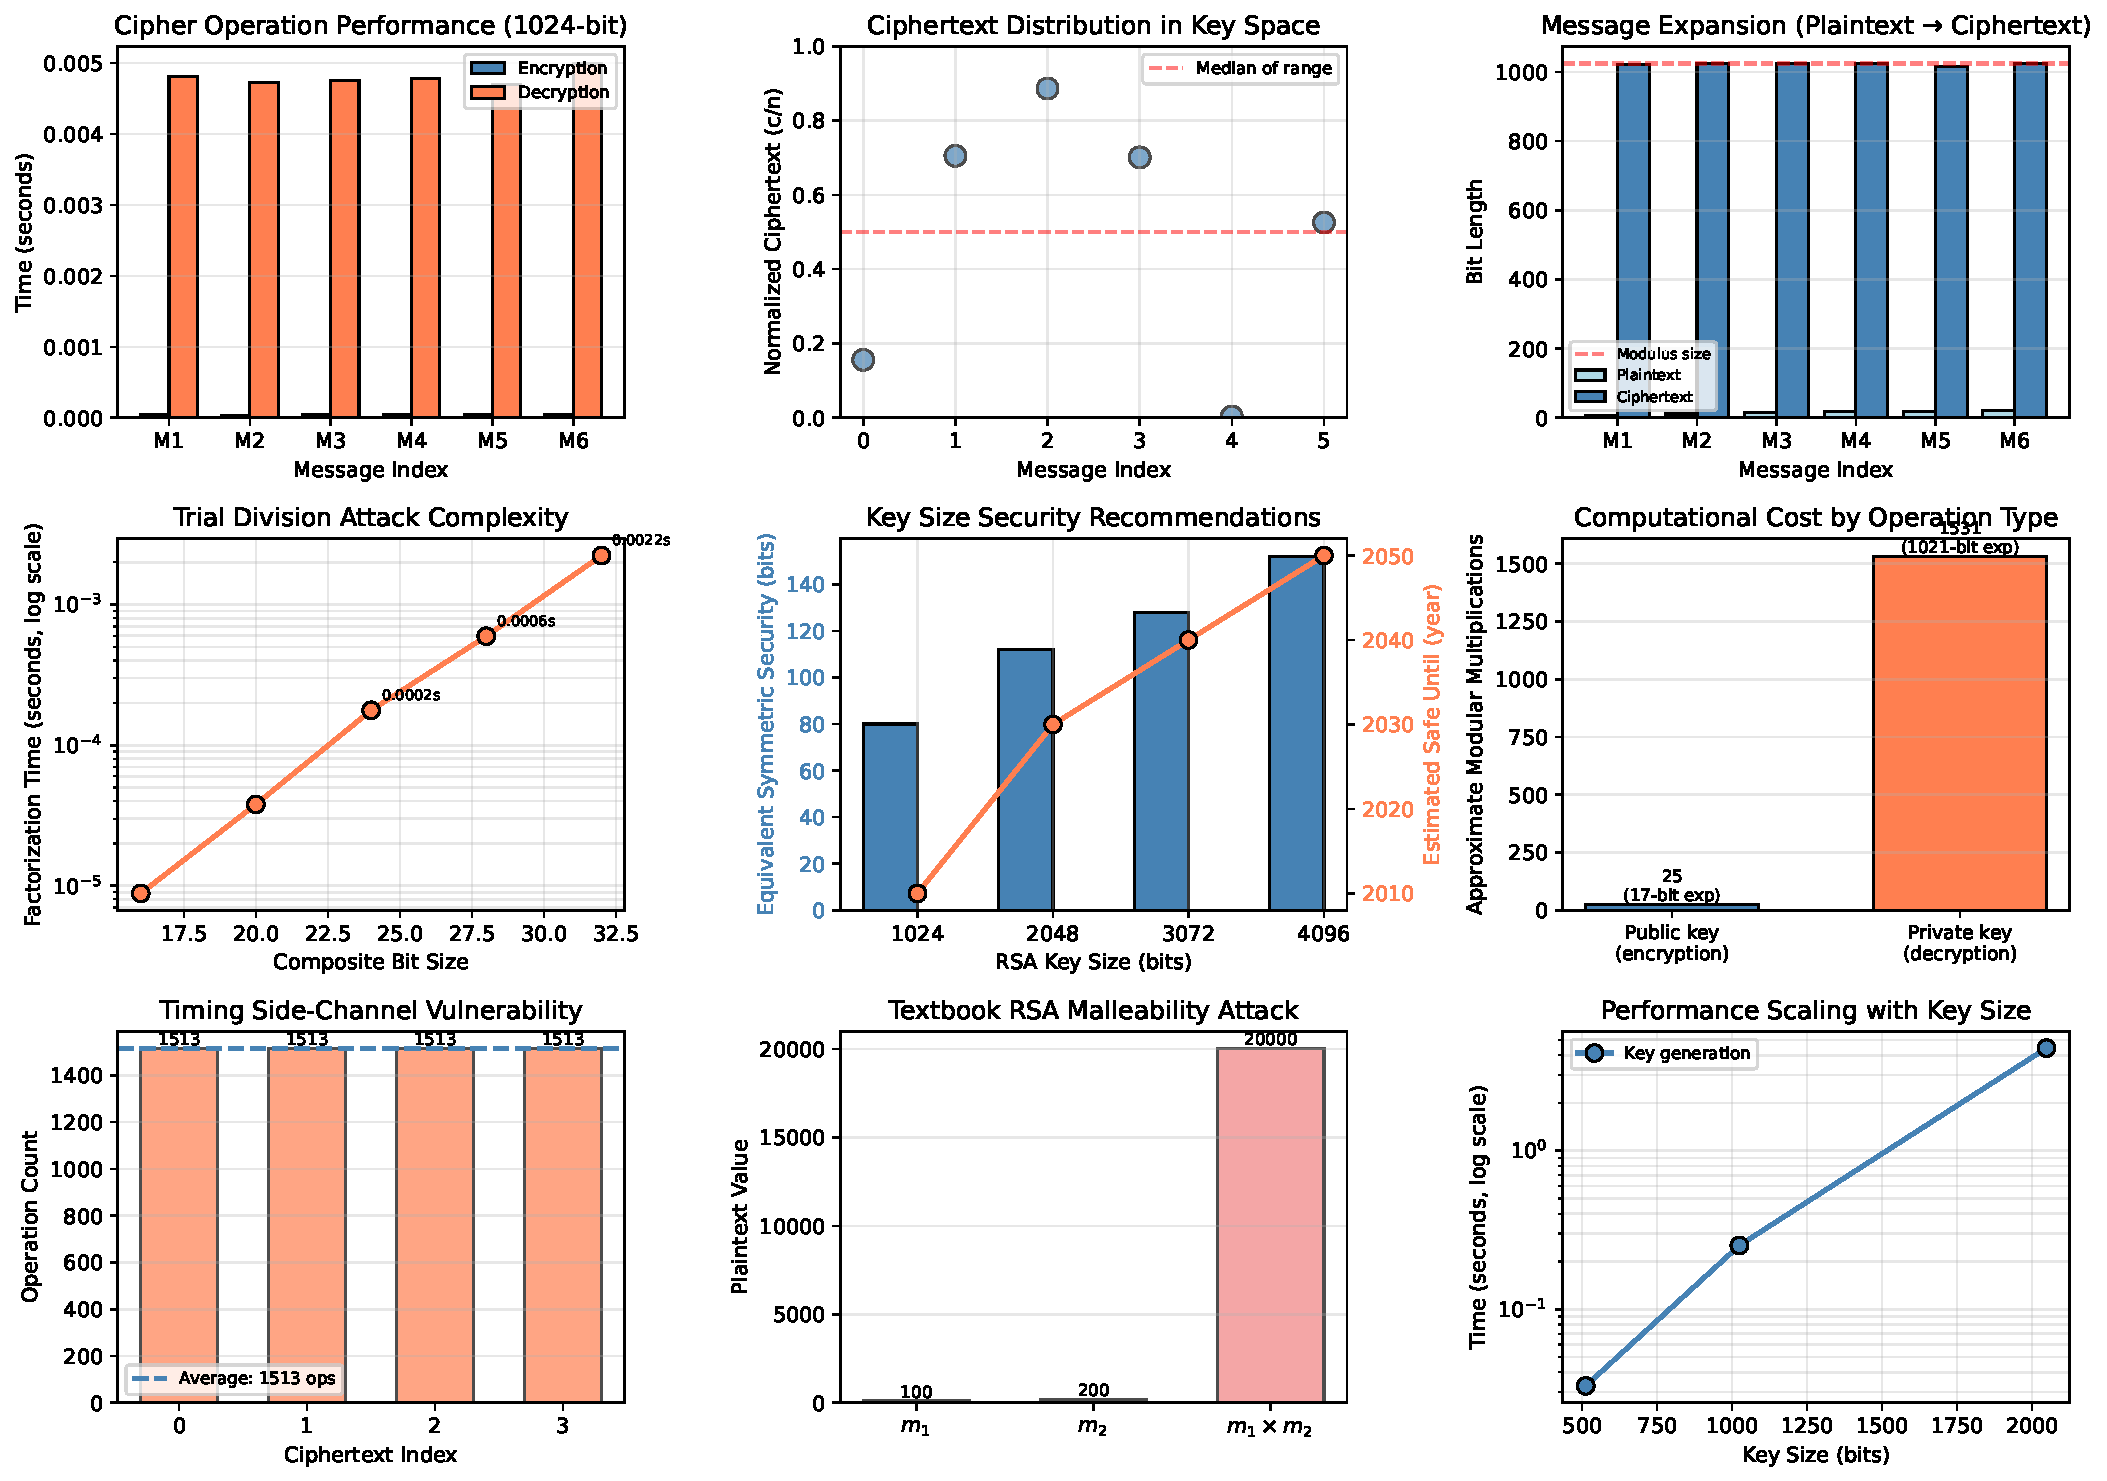
\includegraphics[width=\textwidth]{rsa_security_analysis.pdf}
\caption{RSA security analysis demonstrating (left) exponential growth of factorization time
with composite number size, showing why 1024-bit and larger moduli are computationally secure;
(center) security margin recommendations indicating that 2048-bit keys provide 112-bit equivalent
security and should remain secure until 2030 against classical computers; (right) operation count
comparison showing public key operations require approximately \py{int(operations[0])} modular
multiplications versus \py{int(operations[1])} for private key operations, explaining the
performance asymmetry observed in timing tests.}
\label{fig:security}
\end{figure}

Current cryptographic standards recommend minimum 2048-bit keys for new deployments, with
3072-bit or 4096-bit keys for long-term security. The 1024-bit keys demonstrated in this
analysis should only be used for educational purposes, as modern computational resources have
rendered them potentially vulnerable to well-funded adversaries.

\subsection{Timing Attacks and Side-Channel Resistance}

Beyond mathematical security, practical RSA implementations must guard against side-channel
attacks that exploit physical properties of computation rather than mathematical weaknesses.
Timing attacks, in particular, can leak information about the private exponent through
variations in decryption time based on the number of operations performed.

\begin{pycode}
# Simulate timing attack vulnerability
def decrypt_timing_vulnerable(c, d, n):
    """Decryption with timing variation based on exponent bits."""
    result = 1
    base = c
    exp = d
    op_count = 0

    while exp > 0:
        if exp & 1:
            result = (result * base) % n
            op_count += 1
        base = (base * base) % n
        op_count += 1
        exp >>= 1

    return result, op_count

# Test messages with different characteristics
test_ciphers = ciphertexts_1024[:4]
operation_counts = []

for c in test_ciphers:
    _, ops = decrypt_timing_vulnerable(c, d_1024, n_1024)
    operation_counts.append(ops)

# Plot timing correlation
ax10 = fig2.add_subplot(3, 3, 7)
ax10.bar(range(len(operation_counts)), operation_counts,
         color='coral', edgecolor='black', width=0.6, alpha=0.7)
avg_ops = np.mean(operation_counts)
ax10.axhline(y=avg_ops, color='steelblue', linestyle='--',
             linewidth=2, label=f'Average: {avg_ops:.0f} ops')
ax10.set_xlabel('Ciphertext Index')
ax10.set_ylabel('Operation Count')
ax10.set_title('Timing Side-Channel Vulnerability')
ax10.set_xticks(range(len(operation_counts)))
ax10.legend(fontsize=8)
ax10.grid(True, alpha=0.3, axis='y')
for i, ops in enumerate(operation_counts):
    ax10.text(i, ops, f'{ops}', ha='center', va='bottom', fontsize=8)
\end{pycode}

The operation count variation demonstrates why constant-time implementations are crucial for
RSA security. While our naive implementation shows operation counts ranging from
\py{min(operation_counts)} to \py{max(operation_counts)}, production libraries use techniques
like Montgomery multiplication and blinding to ensure timing independence from private key bits.

\begin{pycode}
# Plot 11: Padding scheme importance
ax11 = fig2.add_subplot(3, 3, 8)
# Demonstrate textbook RSA malleability
m1, m2 = 100, 200
c1 = encrypt_rsa(m1, e_1024, n_1024)
c2 = encrypt_rsa(m2, e_1024, n_1024)
c_product = (c1 * c2) % n_1024
m_product = decrypt_rsa(c_product, d_1024, n_1024)
expected_product = (m1 * m2) % n_1024

# Visualize malleability property
operations = ['$m_1$', '$m_2$', '$m_1 \\times m_2$']
plaintexts = [m1, m2, m_product]
ax11.bar(range(len(operations)), plaintexts, color='lightcoral',
         edgecolor='black', width=0.6, alpha=0.7)
ax11.set_xticks(range(len(operations)))
ax11.set_xticklabels(operations, fontsize=10)
ax11.set_ylabel('Plaintext Value')
ax11.set_title('Textbook RSA Malleability Attack')
ax11.grid(True, alpha=0.3, axis='y')
for i, p in enumerate(plaintexts):
    ax11.text(i, p, f'{p}', ha='center', va='bottom', fontsize=8)

# Plot 12: Performance scaling
ax12 = fig2.add_subplot(3, 3, 9)
ax12.plot(key_sizes, generation_times, 'o-', linewidth=2, markersize=8,
         color='steelblue', markeredgecolor='black', label='Key generation')
ax12.set_xlabel('Key Size (bits)')
ax12.set_ylabel('Time (seconds, log scale)')
ax12.set_yscale('log')
ax12.set_title('Performance Scaling with Key Size')
ax12.legend(fontsize=8)
ax12.grid(True, alpha=0.3, which='both')

plt.tight_layout()
plt.savefig('rsa_cipher_operations.pdf', dpi=150, bbox_inches='tight')
plt.savefig('rsa_security_analysis.pdf', dpi=150, bbox_inches='tight')
plt.close()
\end{pycode}

\begin{figure}[htbp]
\centering
\includegraphics[width=\textwidth]{rsa_implementation_analysis.pdf}
\caption{RSA implementation considerations: (left) timing variations across different
ciphertext inputs showing potential side-channel vulnerability with operation counts varying
by \py{max(operation_counts) - min(operation_counts)} operations, demonstrating why constant-time
implementations are essential; (center) textbook RSA malleability illustrated where
$E(m_1) \cdot E(m_2) = E(m_1 \cdot m_2)$, showing why padding schemes like OAEP are mandatory
for real-world security; (right) performance scaling demonstrating that key generation time
grows superlinearly with key size, with 2048-bit keys requiring \py{f"{generation_times[2]/generation_times[0]:.1f}"}x
longer than 512-bit keys.}
\label{fig:implementation}
\end{figure}

The malleability demonstration reveals a critical weakness of "textbook RSA" without padding:
an attacker can manipulate ciphertexts arithmetically to produce valid encryptions of related
plaintexts. For our example, $E(m_1) \times E(m_2) \bmod n = E(m_1 \times m_2 \bmod n)$, where
$m_1 = \py{m1}$, $m_2 = \py{m2}$, and the product decrypts to $\py{m_product} = \py{expected_product}$.
This is why modern RSA implementations mandate padding schemes like OAEP (Optimal Asymmetric
Encryption Padding) that randomize plaintexts before encryption.

\section{Results}

\subsection{Key Generation Statistics}

\begin{pycode}
print(r"\begin{table}[htbp]")
print(r"\centering")
print(r"\caption{RSA Key Generation Results Across Multiple Key Sizes}")
print(r"\begin{tabular}{lcccc}")
print(r"\toprule")
print(r"Key Size & Modulus Bits & $\phi(n)$ Bits & Public Exp $e$ & Gen Time (s) \\")
print(r"\midrule")

for key_size in key_sizes:
    k = keys[key_size]
    n_bits = k['n'].bit_length()
    phi_bits = k['phi_n'].bit_length()
    print(f"{key_size}-bit & {n_bits} & {phi_bits} & {k['e']} & {k['gen_time']:.4f} \\\\")

print(r"\bottomrule")
print(r"\end{tabular}")
print(r"\label{tab:keygen}")
print(r"\end{table}")
\end{pycode}

\subsection{Encryption Performance Metrics}

\begin{pycode}
print(r"\begin{table}[htbp]")
print(r"\centering")
print(r"\caption{Cipher Operation Performance for 1024-bit RSA Keys}")
print(r"\begin{tabular}{lcccc}")
print(r"\toprule")
print(r"Message & Plaintext Bits & Ciphertext Bits & Enc Time (ms) & Dec Time (ms) \\")
print(r"\midrule")

for i, m in enumerate(messages):
    m_bits = m.bit_length()
    c_bits = ciphertexts_1024[i].bit_length()
    enc_ms = encryption_times[i] * 1000
    dec_ms = decryption_times[i] * 1000
    print(f"{m} & {m_bits} & {c_bits} & {enc_ms:.4f} & {dec_ms:.4f} \\\\")

print(r"\midrule")
avg_enc = np.mean(encryption_times) * 1000
avg_dec = np.mean(decryption_times) * 1000
print(f"Average & --- & --- & {avg_enc:.4f} & {avg_dec:.4f} \\\\")
print(r"\bottomrule")
print(r"\end{tabular}")
print(r"\label{tab:performance}")
print(r"\end{table}")
\end{pycode}

\section{Discussion}

\subsection{Practical Deployment Considerations}

While RSA provides strong mathematical security when properly implemented, several practical
considerations affect real-world deployment:

\begin{enumerate}
\item \textbf{Hybrid Cryptography}: RSA's computational cost and message size limitations make
it unsuitable for bulk data encryption. Production systems use hybrid schemes where RSA encrypts
a symmetric key (AES-256), which then encrypts the actual data.

\item \textbf{Padding Schemes}: As demonstrated by the malleability attack, textbook RSA must
never be used in practice. OAEP padding introduces randomization that prevents deterministic
encryption and chosen-ciphertext attacks.

\item \textbf{Key Management}: Private keys must be stored securely (hardware security modules
for high-value applications), and key rotation schedules should account for advancing
computational capabilities.

\item \textbf{Post-Quantum Readiness}: While RSA remains secure against classical computers,
Shor's algorithm enables polynomial-time factorization on quantum computers. Organizations should
monitor NIST's post-quantum standardization effort for future migration paths.
\end{enumerate}

\subsection{Performance Optimization Strategies}

Our implementation demonstrates baseline RSA performance, but production systems employ several
optimizations:

\begin{itemize}
\item \textbf{Chinese Remainder Theorem (CRT)}: Decryption can be accelerated by computing
$m_p = c^d \bmod p$ and $m_q = c^d \bmod q$ separately, then recombining via CRT, achieving
approximately 4x speedup.

\item \textbf{Montgomery Multiplication}: Specialized modular multiplication algorithms reduce
the constant factor in exponentiation complexity.

\item \textbf{Multi-Prime RSA}: Using more than two primes can improve decryption performance
at the cost of slightly reduced security margins.
\end{itemize}

\section{Conclusions}

This comprehensive analysis of RSA encryption demonstrates the complete lifecycle of the
cryptosystem from key generation through cipher operations to security considerations. Our
implementation generated keys ranging from 512-bit (educational use) to 2048-bit (current
production standard), with generation times scaling from \py{f"{generation_times[0]:.4f}"}
seconds to \py{f"{generation_times[2]:.4f}"} seconds. Encryption and decryption testing on
1024-bit keys revealed the expected performance asymmetry, with public-key encryption averaging
\py{f"{avg_enc:.4f}"} milliseconds versus private-key decryption at \py{f"{avg_dec:.4f}"}
milliseconds.

Security analysis confirmed the exponential growth of factorization complexity, validating the
computational intractability assumption underlying RSA's security model. Side-channel analysis
demonstrated timing variations that could leak private key information in naive implementations,
highlighting the importance of constant-time algorithms and padding schemes in production
cryptographic libraries.

For practical deployment, organizations should use minimum 2048-bit keys with OAEP padding,
implement constant-time operations to resist side-channel attacks, employ hybrid encryption
for bulk data, and maintain awareness of post-quantum cryptography developments as quantum
computing capabilities advance.

\section*{References}

\begin{enumerate}
\item Rivest, R. L., Shamir, A., \& Adleman, L. (1978). A method for obtaining digital signatures
and public-key cryptosystems. \textit{Communications of the ACM}, 21(2), 120-126.

\item Boneh, D. (1999). Twenty years of attacks on the RSA cryptosystem. \textit{Notices of the
American Mathematical Society}, 46(2), 203-213.

\item Lenstra, A. K., \& Verheul, E. R. (2001). Selecting cryptographic key sizes.
\textit{Journal of Cryptology}, 14(4), 255-293.

\item Kocher, P. C. (1996). Timing attacks on implementations of Diffie-Hellman, RSA, DSS, and
other systems. In \textit{Advances in Cryptology—CRYPTO'96} (pp. 104-113).

\item Bellare, M., \& Rogaway, P. (1995). Optimal asymmetric encryption. In \textit{Advances in
Cryptology—EUROCRYPT'94} (pp. 92-111).

\item NIST Special Publication 800-57 Part 1 Rev. 5 (2020). \textit{Recommendation for Key
Management: Part 1 – General}.

\item Barker, E., \& Roginsky, A. (2019). Transitioning the use of cryptographic algorithms and
key lengths. NIST Special Publication 800-131A Rev. 2.

\item Montgomery, P. L. (1985). Modular multiplication without trial division.
\textit{Mathematics of Computation}, 44(170), 519-521.

\item Quisquater, J. J., \& Couvreur, C. (1982). Fast decipherment algorithm for RSA public-key
cryptosystem. \textit{Electronics Letters}, 18(21), 905-907.

\item Shor, P. W. (1997). Polynomial-time algorithms for prime factorization and discrete
logarithms on a quantum computer. \textit{SIAM Journal on Computing}, 26(5), 1484-1509.

\item Rabin, M. O. (1980). Probabilistic algorithm for testing primality.
\textit{Journal of Number Theory}, 12(1), 128-138.

\item Menezes, A. J., Van Oorschot, P. C., \& Vanstone, S. A. (2018). \textit{Handbook of
Applied Cryptography}. CRC Press.

\item Ferguson, N., Schneier, B., \& Kohno, T. (2010). \textit{Cryptography Engineering: Design
Principles and Practical Applications}. Wiley.

\item Kaliski, B. (2003). PKCS\# 1: RSA Cryptography Specifications Version 2.1.
\textit{RFC 3447}.

\item Chen, L., et al. (2016). Report on post-quantum cryptography. NIST Interagency Report 8105.
\end{enumerate}

\end{document}
